\documentclass{article}
\usepackage[T1]{fontenc}
\usepackage{lmodern}
\usepackage{graphicx}
\usepackage{amsmath,amssymb}
\usepackage[a4paper,margin=2cm]{geometry}
\usepackage[absolute,overlay]{textpos}
\setlength{\TPHorizModule}{1mm}
\setlength{\TPVertModule}{1mm}
\usepackage[indonesian]{babel}
\usepackage{hyperref}
\setlength{\emergencystretch}{2em}
% unit: Halaman 16

\begin{document}

% === Halaman 16 (llm) ===

\vspace{175.23mm}

\section*{Program Python untuk enkripsi-dekripsi file dengan cipher XOR sederhana}

\vspace{10mm}

% deskripsi: Screenshot kode program Python untuk fungsi xor_cipher_encrypt
% bbox normalisasi: [0.0100, 0.2200, 0.5000, 0.8100]
\begin{textblock*}{102.90mm}(2.10mm,65.34mm)
\noindent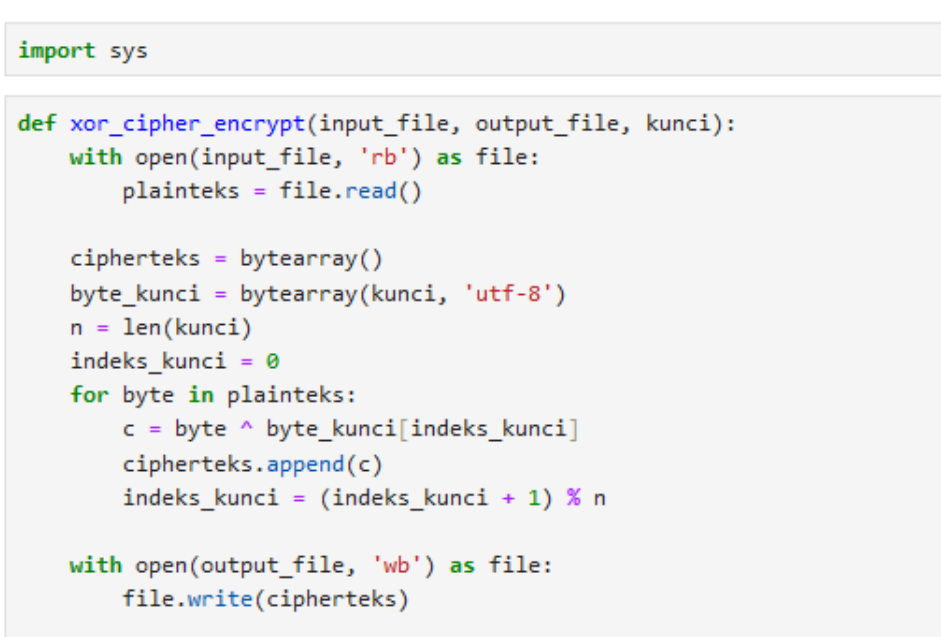
\includegraphics[width=102.90mm,height=175.23mm]{../../images/llm/page_016_img_01.png}%
\end{textblock*}

% deskripsi: Screenshot kode program Python untuk fungsi xor_cipher_decrypt
% bbox normalisasi: [0.5100, 0.2200, 0.9900, 0.8100]
\begin{textblock*}{100.80mm}(107.10mm,65.34mm)
\noindent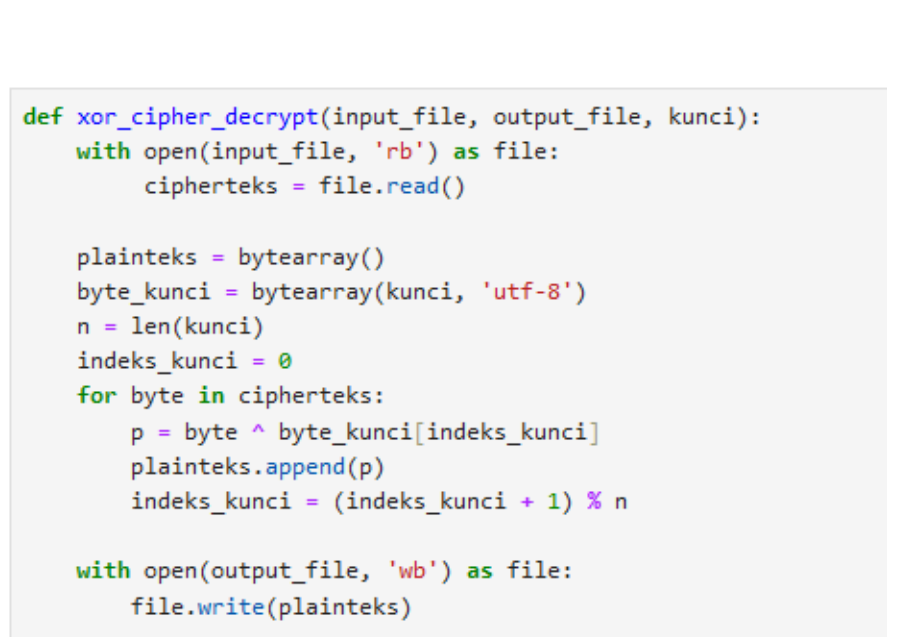
\includegraphics[width=100.80mm,height=175.23mm]{../../images/llm/page_016_img_02.png}%
\end{textblock*}

\end{document}
